\documentclass[aspectratio=169,10pt]{beamer}

\usetheme{metropolis}
\usepackage{appendixnumberbeamer}
\usepackage{booktabs}
\usepackage[scale=2]{ccicons}
\usepackage{pgfplots}
\usepgfplotslibrary{dateplot}
\usepackage{xspace}
\usepackage{tikz}
\usetikzlibrary{mindmap,trees,shapes,arrows,positioning,pie}
\usepackage{tcolorbox}

\title{Guide to Pursuing a Computer Science PhD in Europe (Germany Focus)}
\subtitle{Talk 2: PhD Life and Beyond}
\date{\today}
\author{Dr. Bijun Li}
\institute{Expert in International Computer Science Research}

\begin{document}

\maketitle

\begin{frame}{Overview of Talk 2}
    \begin{itemize}
        \item Funding and Financial Planning
        \item Starting Your PhD and Research Life
        \item Publishing and Conferences
        \item Challenges and Professional Development
        \item Completing Your PhD
        \item Career Prospects Post-PhD
    \end{itemize}
\end{frame}

\begin{frame}{Funding and Financial Planning}
    \begin{columns}[T]
        \begin{column}{0.5\textwidth}
            \textbf{Types of Funding}
            \begin{itemize}
                \item University positions (wissenschaftlicher Mitarbeiter)
                \item Scholarships (e.g., DAAD, DFG)
                \item Industry-sponsored PhDs
            \end{itemize}
            
            \textbf{Stipends vs. Employment}
            \begin{itemize}
                \item Stipends: Tax-free, no social security
                \item Employment: Taxed, includes benefits
            \end{itemize}
        \end{column}
        \begin{column}{0.5\textwidth}
            \textbf{Living Costs}
            \begin{itemize}
                \item Vary by city (e.g., Munich vs. Leipzig)
                \item Rent: 30-40% of income
                \item Food, insurance, transportation
            \end{itemize}
            
            \textbf{Budgeting Tips}
            \begin{itemize}
                \item Use student discounts
                \item Plan for conference travel
                \item Consider part-time work options
            \end{itemize}
        \end{column}
    \end{columns}
\end{frame}

\begin{frame}{Starting Your PhD}
    \textbf{Arrival and Settlement}
    \begin{itemize}
        \item Finding accommodation (university housing, WGs)
        \item Administrative tasks (Anmeldung, bank account, visa)
        \item Health insurance (public vs. private)
    \end{itemize}
    
    \textbf{Integration into Research Group}
    \begin{itemize}
        \item Attend orientation programs
        \item Meet colleagues and supervisors
        \item Understand lab protocols and resources
    \end{itemize}
    
    \textbf{Developing Your Research Plan}
    \begin{itemize}
        \item Conduct thorough literature review
        \item Define clear research questions
        \item Select appropriate methodologies
        \item Set realistic milestones
    \end{itemize}
\end{frame}

\begin{frame}{PhD Life and Research}
    \begin{columns}[T]
        \begin{column}{0.5\textwidth}
            \textbf{Structuring Your Research}
            \begin{itemize}
                \item Set milestones and deadlines
                \item Regular supervisor meetings
                \item Balance research and other duties
            \end{itemize}
            
            \textbf{Collaboration Opportunities}
            \begin{itemize}
                \item Within your research group
                \item Interdisciplinary projects
                \item International collaborations
            \end{itemize}
        \end{column}
        \begin{column}{0.5\textwidth}
            \textbf{Teaching and Supervision}
            \begin{itemize}
                \item Teaching assistant duties
                \item Supervise bachelor's/master's theses
                \item Develop pedagogical skills
            \end{itemize}
            
            \textbf{Work-Life Balance}
            \begin{itemize}
                \item Manage time effectively
                \item Engage in non-academic activities
                \item Utilize university sports/clubs
            \end{itemize}
        \end{column}
    \end{columns}
\end{frame}

\begin{frame}{Publishing and Conferences}
    \textbf{Importance of Publications in CS}
    \begin{itemize}
        \item Conference papers often valued over journals
        \item Build your research profile
    \end{itemize}
    
    \textbf{Choosing the Right Venues}
    \begin{itemize}
        \item Top conferences: ICML, NeurIPS, CVPR, SIGCOMM
        \item Relevant workshops for early-stage research
    \end{itemize}
    
    \textbf{Writing and Submission Process}
    \begin{itemize}
        \item Use collaborative writing tools
        \item Understand peer review process
        \item Handle revisions and rejections constructively
    \end{itemize}
    
    \textbf{Presenting at Conferences}
    \begin{itemize}
        \item Prepare effective presentations
        \item Network with other researchers
        \item Gain visibility in your field
    \end{itemize}
\end{frame}

\begin{frame}{Challenges and Professional Development}
    \begin{columns}[T]
        \begin{column}{0.5\textwidth}
            \textbf{Common Challenges}
            \begin{itemize}
                \item Imposter syndrome
                \item Research setbacks
                \item Work-life balance
                \item Cultural adaptation
            \end{itemize}
            
            \textbf{Overcoming Challenges}
            \begin{itemize}
                \item Seek support (supervisor, peers)
                \item Attend workshops on research skills
                \item Practice self-care and mindfulness
            \end{itemize}
        \end{column}
        \begin{column}{0.5\textwidth}
            \textbf{Professional Development}
            \begin{itemize}
                \item Enhance technical skills
                \item Develop soft skills (communication, leadership)
                \item Explore internship opportunities
                \item Engage in entrepreneurship programs
            \end{itemize}
            
            \textbf{Networking}
            \begin{itemize}
                \item Attend summer schools
                \item Join professional associations
                \item Utilize online platforms (LinkedIn, ResearchGate)
            \end{itemize}
        \end{column}
    \end{columns}
\end{frame}

\begin{frame}{Completing Your PhD}
    \textbf{Thesis Writing Process}
    \begin{itemize}
        \item Start early, write continuously
        \item Follow university guidelines
        \item Seek feedback regularly
    \end{itemize}
    
    \textbf{Submission and Defense}
    \begin{itemize}
        \item Understand submission requirements
        \item Prepare for oral defense (disputation)
        \item Typical duration: 60-90 minutes
    \end{itemize}
    
    \textbf{Publication Requirements}
    \begin{itemize}
        \item Vary by university and department
        \item Often 3-4 conference papers or 1-2 journal articles
    \end{itemize}
    
    \textbf{Timelines}
    \begin{itemize}
        \item Average duration: 3-5 years
        \item Extensions possible if needed
    \end{itemize}
\end{frame}

\begin{frame}{Career Prospects Post-PhD}
    \begin{columns}[T]
        \begin{column}{0.5\textwidth}
            \textbf{Academic Paths}
            \begin{itemize}
                \item Postdoctoral positions
                \item Junior professorships
                \item Research group leaders
            \end{itemize}
            
            \textbf{Industry Opportunities}
            \begin{itemize}
                \item R\&D roles in tech companies
                \item Data science positions
                \item AI/ML specialists
            \end{itemize}
        \end{column}
        \begin{column}{0.5\textwidth}
            \textbf{Research Positions}
            \begin{itemize}
                \item Government research institutes
                \item Industrial research labs
                \item Think tanks and consultancies
            \end{itemize}
            
            \textbf{Entrepreneurship}
            \begin{itemize}
                \item Tech startups
                \item University spin-offs
                \item Consulting services
            \end{itemize}
        \end{column}
    \end{columns}
    
    \textbf{International Job Market}
    \begin{itemize}
        \item Strong demand for CS PhDs globally
        \item Opportunities in EU, US, Asia
    \end{itemize}
\end{frame}

\begin{frame}{Resources and Support}
    \textbf{University Services}
    \begin{itemize}
        \item Career centers
        \item International offices
        \item Mental health support
    \end{itemize}
    
    \textbf{Professional Networks}
    \begin{itemize}
        \item Gesellschaft für Informatik (GI)
        \item IEEE Computer Society
        \item ACM SIGCSE
    \end{itemize}
    
    \textbf{Online Resources}
    \begin{itemize}
        \item Research portals (e.g., ResearchGate)
        \item CS-specific forums and communities
        \item DAAD (German Academic Exchange Service) website
    \end{itemize}
    
    \textbf{Mentoring Programs}
    \begin{itemize}
        \item University-led mentoring
        \item Industry mentorship opportunities
    \end{itemize}
\end{frame}

\begin{frame}{Conclusion}
    \textbf{Key Takeaways}
    \begin{itemize}
        \item Plan finances carefully
        \item Embrace the research journey
        \item Publish and present your work
        \item Develop a strong professional network
        \item Prepare for diverse career paths
    \end{itemize}
    
    \textbf{Final Advice}
    \begin{itemize}
        \item Stay curious and passionate about your research
        \item Be open to interdisciplinary collaborations
        \item Embrace challenges as growth opportunities
        \item Maintain a healthy work-life balance
    \end{itemize}
\end{frame}

\begin{frame}{Q\&A Session}
    \centering
    \large{Time for Your Questions!}
    
    \vspace{1cm}
    
    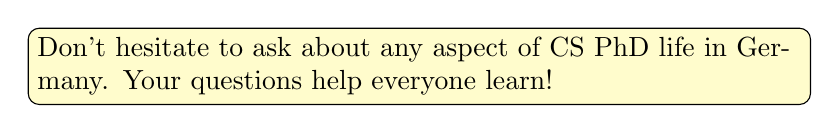
\begin{tikzpicture}
        \node[draw,rounded corners,fill=yellow!20,text width=0.8\textwidth] {
            Don't hesitate to ask about any aspect of CS PhD life in Germany. Your questions help everyone learn!
        };
    \end{tikzpicture}
\end{frame}

\end{document}